\section{Validation}

\subsection{5-Pins Simulation Setup}
The proposed controller was first evaluated in a 5-pins lane-change simulation. The reference path contains five consecutive double-lane-change maneuvers with the same lateral displacement of 3.5 m and progressively shorter maneuver durations, starting from 4 s. This setting produces a continuous risk gradient: the first two double lane changes are mild, the third is transitional, and the fourth and fifth contain strong lateral excitation. The controlled object follows the semi-trailer tank truck setting used in TruckSim validation, while the Q-band module only uses the predicted lateral-acceleration sequence in the controller.

Fifteen controller variants were compared, including baseline tracking, lateral-acceleration hard constraint, acceleration magnitude/difference penalties, fixed Q-band, preview-adaptive Q-band, feedback-assisted Q-band, and Q-band soft constraints. The main metrics are peak $|\LTR_{\mathrm{est}}|$, RMS LTR, peak lateral acceleration, RMS tracking error, and segment-wise tracking/safety indicators.

\begin{figure*}[!t]
\centering
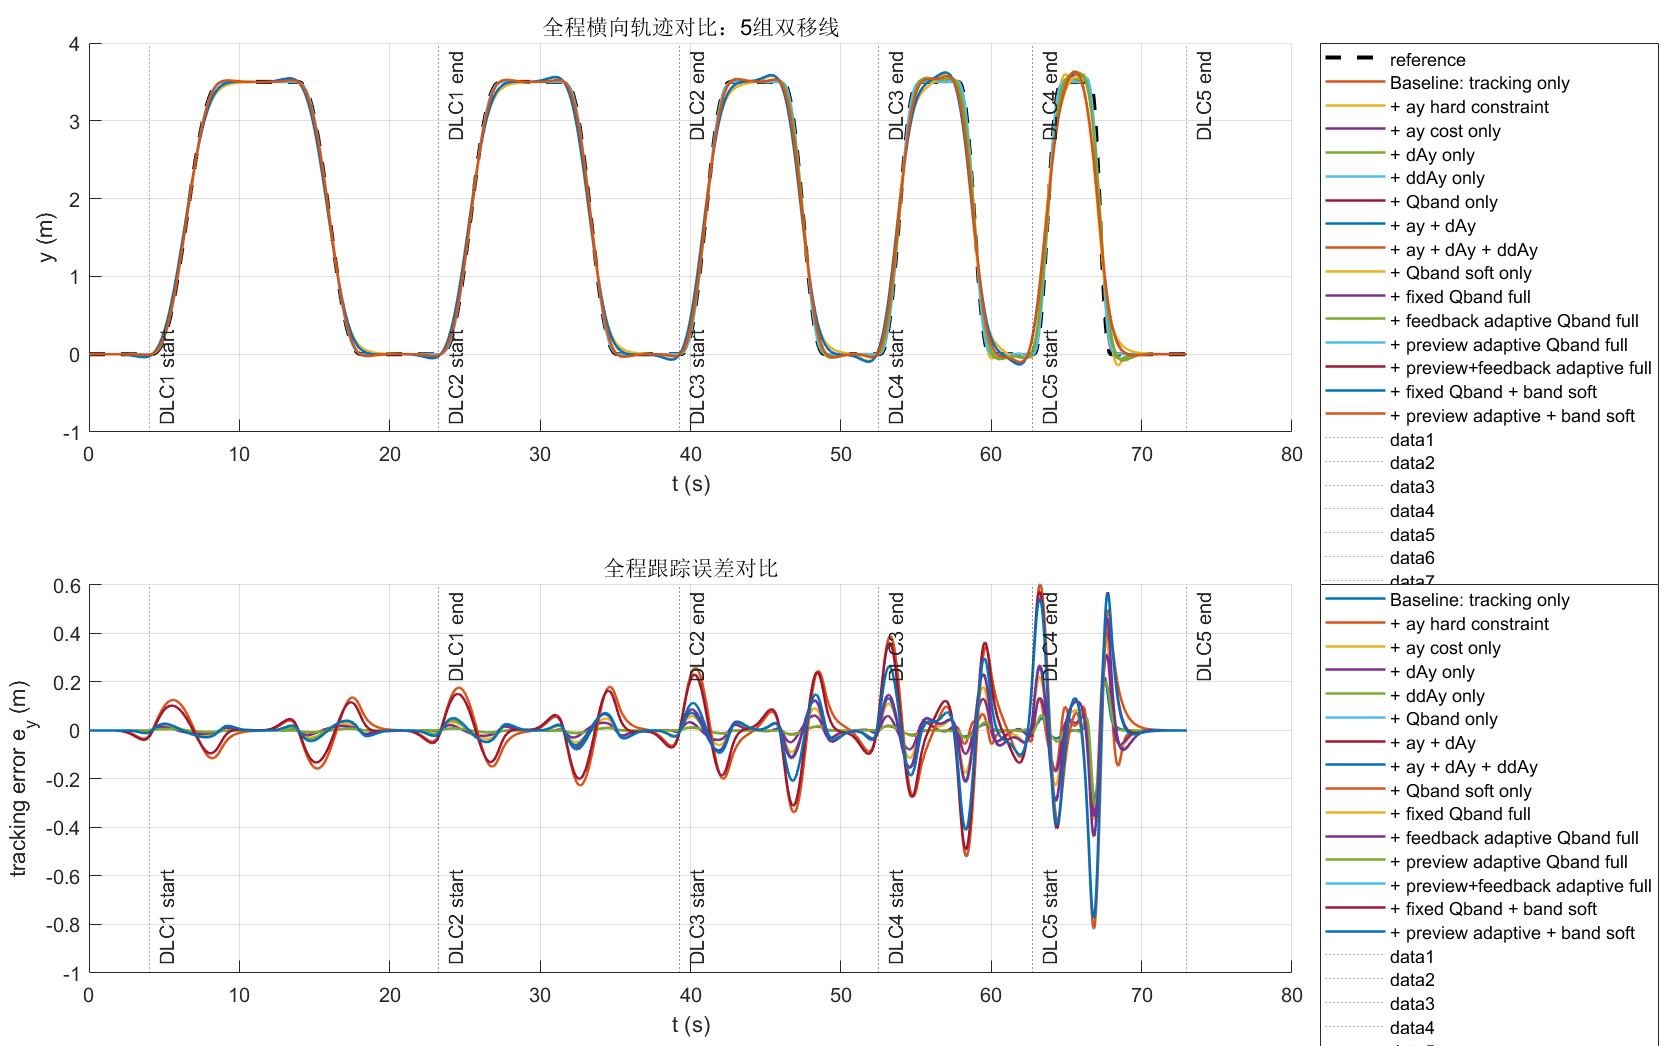
\includegraphics[width=0.98\textwidth]{fig/results1.png}
\caption{Five-pins tracking results. Low-risk segments are tracked closely by all methods; in the high-risk DLC4--DLC5 segments, Q-band and soft-constraint variants intentionally allow moderate path deviation to reduce rollover excitation.}
\label{fig:fivepins_tracking}
\end{figure*}
% TODO（作者）：当前 results1.png 是 MATLAB 粗图。建议最终版只保留 reference、baseline、fixed Q-band、preview Q-band、preview Q-band + soft 四条曲线；删除 data1/data2 等无效 legend；英文坐标轴和标题；用竖向浅色背景块标注 DLC1--DLC5，避免密集虚线和旋转文字。

\subsection{Simulation Results}
Fig.~\ref{fig:fivepins_tracking} shows that all controllers track the first three maneuvers with small errors. As the maneuver duration decreases, the baseline tracker maintains path accuracy but injects stronger oscillatory lateral acceleration. Q-band methods begin to relax tracking in DLC4 and DLC5, especially near the lane-return phases, where the predicted acceleration would otherwise fall into the critical band. The largest temporary tracking deviation is approximately xxx m in the current simulation and remains acceptable for the intended emergency maneuver envelope.

\begin{figure*}[!t]
\centering
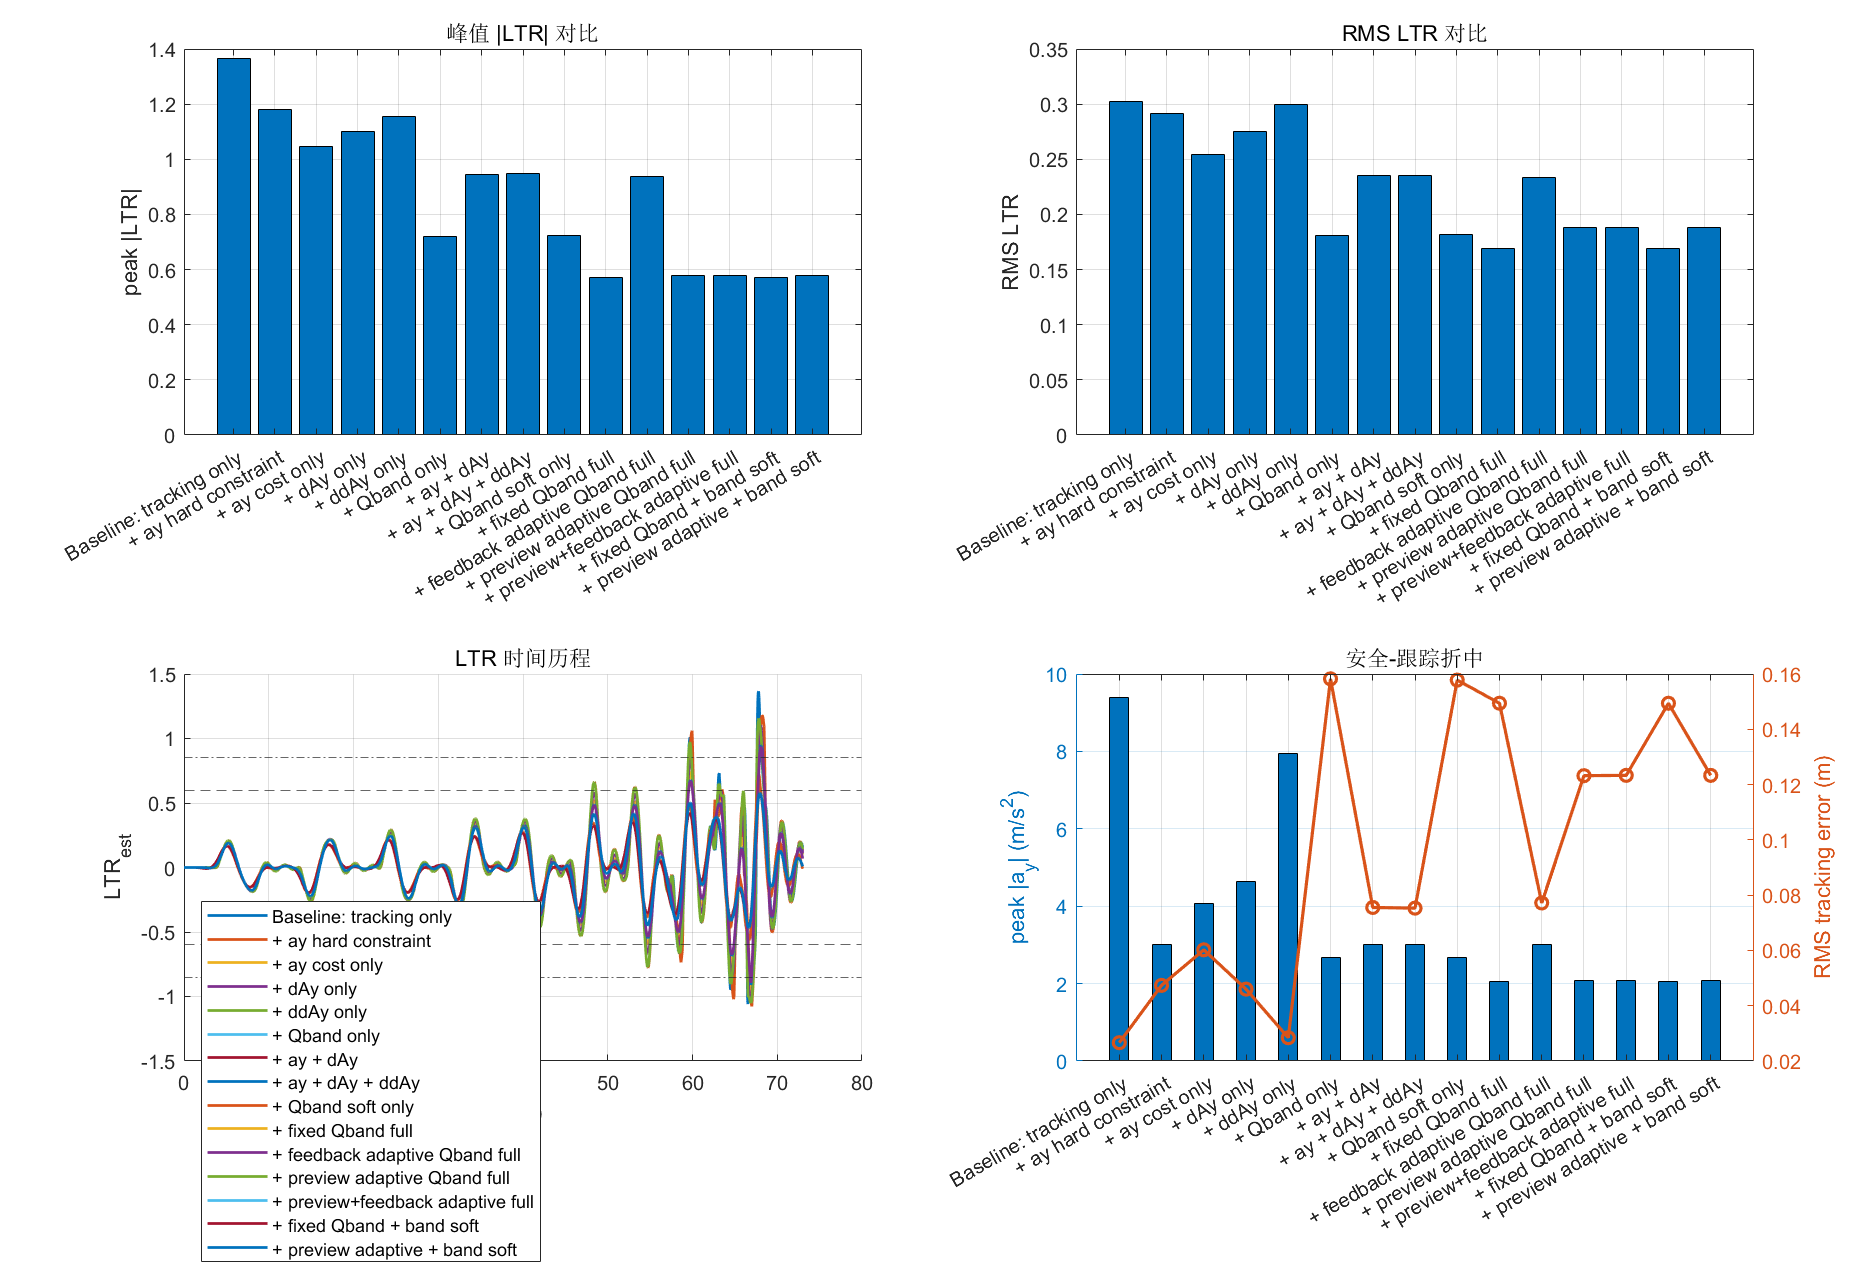
\includegraphics[width=0.98\textwidth]{fig/results2.png}
\caption{Ablation summary for the 5-pins simulation. Q-band-based variants reduce both peak $|\LTR_{\mathrm{est}}|$ and RMS LTR compared with baseline tracking, while the safety improvement is obtained at the cost of controlled tracking relaxation.}
\label{fig:fivepins_ablation}
\end{figure*}
% TODO（作者）：当前 results2.png 信息量太大。建议最终拆成两张或一个 2x2 组合图：peak |LTR|、RMS LTR、selected LTR time histories、safety-tracking Pareto。横轴 case 名称需要缩短，例如 Base、AyLim、Qband、Pre-Q、Pre-Q+Soft；安全阈值线建议统一标为 warning/danger。

The ablation results in Fig.~\ref{fig:fivepins_ablation} show three trends. First, the baseline peak $|\LTR_{\mathrm{est}}|$ reaches about xxx, exceeding the rollover-risk limit. Second, acceleration magnitude and difference penalties reduce part of the risk but cannot consistently suppress the critical high-risk segments. Third, fixed or adaptive Q-band variants reduce peak $|\LTR_{\mathrm{est}}|$ to approximately xxx--xxx and lower RMS LTR from xxx to xxx. The preview-adaptive and soft-constraint variants provide the most consistent reduction because the weights rise before DLC4--DLC5 and the optimizer is discouraged from placing energy in the critical band.

\begin{figure*}[!t]
\centering
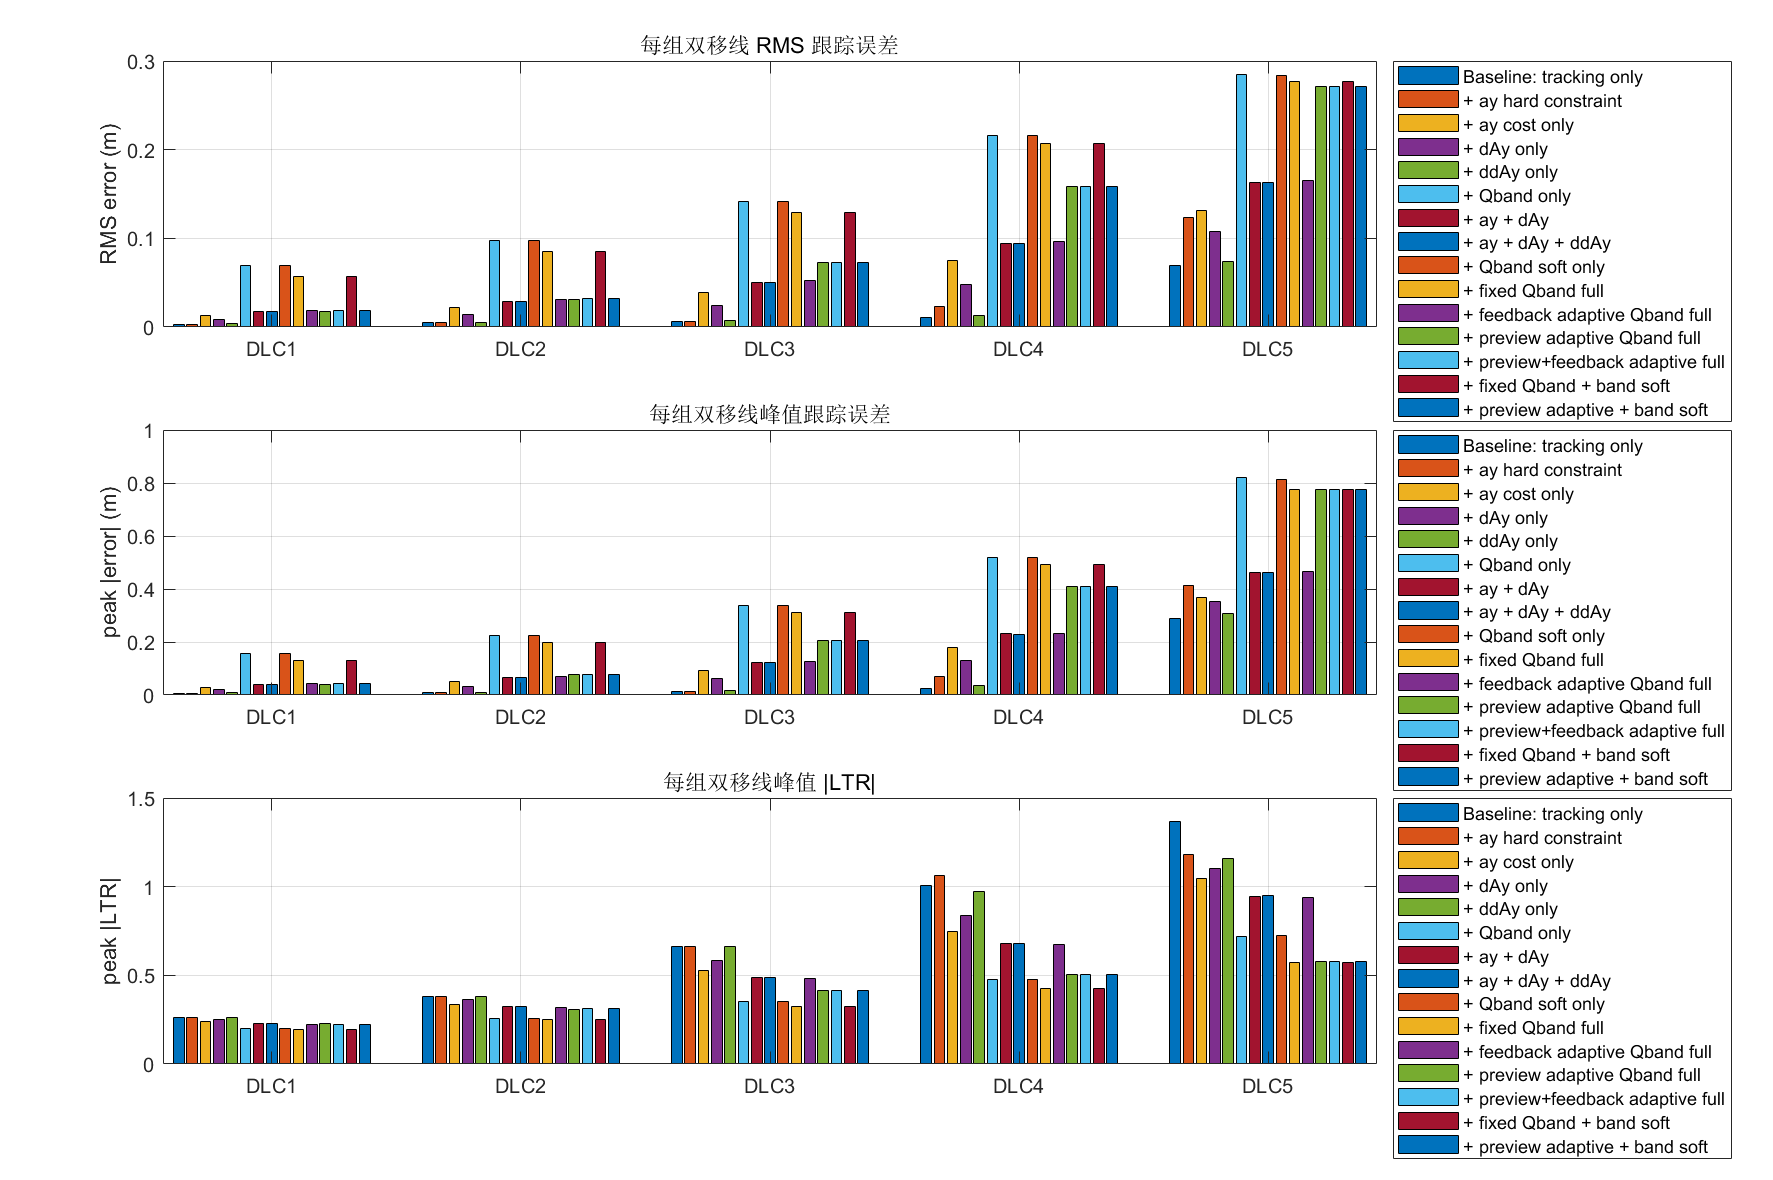
\includegraphics[width=0.98\textwidth]{fig/results3.png}
\caption{Segment-wise 5-pins metrics. The difference among methods is small in DLC1--DLC2, becomes visible in DLC3, and is dominated by the safety-tracking tradeoff in DLC4--DLC5.}
\label{fig:fivepins_segments}
\end{figure*}
% TODO（作者）：当前 results3.png legend 过大且重复三次。建议最终用分组柱状图只展示 4--5 个代表 case，并将 legend 放在图外上方一行；如果篇幅不够，可只保留第三行“每组双移线峰值 |LTR|”，把误差指标放入表格。

Segment-wise results in Fig.~\ref{fig:fivepins_segments} further confirm that Q-band ART is mainly activated in the dangerous sections. In DLC1 and DLC2, all methods have similar peak $|\LTR|$ and tracking error. In DLC3 the Q-band methods begin to separate from acceleration-only regularization. In DLC4 and DLC5, the baseline and acceleration-only strategies approach or exceed the risk threshold, while Q-band variants keep the peak risk proxy near xxx. This supports the design goal: low-risk segments remain close to ordinary tracking, and high-risk segments are reshaped to suppress dangerous lateral excitation.

\subsection{Model-Truck Experiment}
The 1:14 semi-trailer tank truck experiment was conducted to verify that the Q-band mechanism remains effective on a physical platform. The experiment used a double-lane-change or 5-pins-like reference path scaled according to the model-truck operating envelope. Baseline tracking and Q-band ART were compared under the same speed and filling-rate settings. The measured responses include path tracking, steering command, lateral acceleration, roll/yaw response, liquid-surface motion when available, and controller solve time.

The model-truck results show the same qualitative behavior as the simulation. Baseline tracking follows the reference more tightly but excites larger roll-slosh motion, and the anti-roll support/contact or rollover-risk proxy reaches xxx. Q-band ART reduces the peak risk proxy by xxx\%, keeps the liquid/roll response within xxx, and increases RMS tracking error from xxx m to xxx m. The controller average and peak solve times are xxx ms and xxx ms, respectively, satisfying the real-time requirement of the experimental platform.

% TODO（作者）：这里后续需要插入模型车实验总图。建议包含：平台照片、实验路径、baseline vs Q-band 轨迹、风险代理/LTR、液面或侧倾响应、求解时间。若没有液面可靠识别，就明确写“liquid-surface motion is used only for qualitative video confirmation”。

\begin{table}[!t]
\caption{Validation Summary With Replaceable Results}
\label{tab:validation_summary}
\centering
\begin{tabularx}{\linewidth}{lXXX}
\toprule
Case & Peak risk proxy & RMS error & Solve time\\
\midrule
Simulation baseline & xxx & xxx m & xxx ms\\
Simulation Q-band ART & xxx & xxx m & xxx ms\\
Model-truck baseline & xxx & xxx m & --\\
Model-truck Q-band ART & xxx & xxx m & xxx ms\\
\bottomrule
\end{tabularx}
\end{table}
% TODO（作者）：表中 peak risk proxy 最终统一成 peak |LTR_est|、peak roll rate 或 support-contact indicator 之一；仿真和模型车如果指标不同，需要在表注里说明，避免直接比较不同定义的数值。
